\documentclass[10pt,a4paper]{article}
\usepackage[utf8]{inputenc}
\usepackage{amsmath}
\usepackage{amsfonts}
\usepackage{amssymb}
\usepackage{natbib}
\usepackage{graphicx}
\usepackage[left=2cm,right=2cm,top=2cm,bottom=2cm]{geometry}
\begin{document}

We discuss a method to smooth observed data, $u_\mathrm{obs}$, which can be spatial, temporal, or higher dimensional data, and the observations are generally irregularly spaced.  Methods which handle this task often fall in at least one of two catagories.  One approach is to fit a set of basis functions to the observations using least-squares or regularized least-squares \citep[e.g.][]{Fasshauer2007}.  Smoothing splines can be viewed in this context where the basis functions being fit to the observation are polyharmonic splines.  The second catagory is Gaussian process regression, which is a Bayesian technique where a stochastic prior model is assumed for the underlying signal \citep[e.g.][]{Rasmussen2006}.  Kriging is among the better known examples of Gaussian process regression.  The two approaches are not always distinct.  For example, \citet{Kimeldorf1970} showed that smoothing splines can be cast as a Bayesian estimation problem with the appropriate stochastic prior model.  Our method is an example of Gaussian process regression where our smoothed solution, $u_\mathrm{post}$, incorporates $u_\mathrm{obs}$ and a stochastic prior model for the underlying signal which we are trying to recover.  We constrain $u_\mathrm{post}$ with the observation equation

\begin{equation}\label{eq:Data}
  u_\mathrm{post} = u_\mathrm{obs} + \epsilon,\ \ \ \epsilon \sim \mathcal{N}(0,\mathbf{C}_\mathrm{obs}),
\end{equation}
and the prior model

\begin{equation}\label{eq:Prior}
  u_\mathrm{prior} \sim \mathcal{N}(0,\mathbf{C}_\mathrm{prior}),
\end{equation}
where $\epsilon$ and $u_\mathrm{prior}$ are considered to be Gaussian processes with zero mean and covariances $\mathbf{C}_\mathrm{obs}$ and $\mathbf{C}_\mathrm{prior}$ respectively.  The solution for $u_\mathrm{post}$ minimizes the objective function  

\begin{equation}\label{eq:Objective}
||u_\mathrm{post} - u_\mathrm{obs}||_{\mathbf{C}_\mathrm{obs}}^2 + 
||u_\mathrm{post}||_{\mathbf{C}_\mathrm{prior}}^2
\end{equation}
and is itself a Gaussian process with a distribution described by

\begin{equation}
  u_\mathrm{post} \sim \mathcal{N}(\bar{u}_\mathrm{post},\mathbf{C}_\mathrm{post}).
\end{equation}
We use $\bar{u}_\mathrm{post}$ and $\mathbf{C}_\mathrm{post}$ to denote the mean and covariance of $u_\mathrm{post}$ respectively.  Using Bayesian linear regression \citep[e.g.][]{Tarantola2005} these values are found to be  

\begin{equation}\label{eq:GeneralSolution}
\begin{split}
  \bar{u}_\mathrm{post} &= (\mathbf{C}_\mathrm{obs}^{-1} + 
                            \mathbf{C}_\mathrm{prior}^{-1})^{-1}
                            \mathbf{C}_\mathrm{obs}^{-1} u_\mathrm{obs}
\\
\mathbf{C}_\mathrm{post} &= (\mathbf{C}_\mathrm{obs}^{-1} + 
                             \mathbf{C}_\mathrm{prior}^{-1})^{-1}.                          
\end{split}
\end{equation}
 
$\mathbf{C}_\mathrm{obs}$ is presumably well known, while $\mathbf{C}_\mathrm{prior}$ needs to be chosen based on an understanding of the underlying signal which we are trying to estimate.  With a judicious choice of $\mathbf{C}_\mathrm{prior}$,  eq. (\ref{eq:GeneralSolution}) can be made equivalent to several well established smoothing methods.  In particular, we demonstrate how eq. (\ref{eq:GeneralSolution}) can be viewed as a low-pass filter with a well defined cutoff frequency. This is first demonstrated for filtering one-dimensional data, and the extension to higher dimensions follows naturally.  

\section*{One-dimensional smoothing}
For one-dimensional data we consider a prior which can be stated implicitly as

\begin{equation}\label{eq:ImplicitPrior1D}
  \mathbf{D}_{n} u_\mathrm{prior} = q, \ \ \ q \sim \mathcal{N}(0,\lambda^2),
\end{equation}  
where $\mathbf{D}_n$ is an $n$'th order differentiation matrix, and $q$ is white noise with constant variance $\lambda^2$.  If we momentarily ignore the fact that $\mathbf{D}_n$ is not invertible then we can explicitly write our prior covariance as

\begin{equation}\label{eq:ExplicitPrior1D}
\mathbf{C_\mathrm{prior}} = \lambda^2(\mathbf{D}_n^T\mathbf{D}_n)^{-1},
\end{equation}
and the filtered mean and covariance are described by
\begin{equation}\label{eq:1DSolution}
\begin{split}
\bar{u}_\mathrm{post} &= (\mathbf{C}_\mathrm{obs}^{-1} +   
                   \frac{1}{\lambda^2}\mathbf{D}_n^T\mathbf{D}_n)^{-1}\mathbf{C}_\mathrm{obs}^{-1}
                   u_\mathrm{obs}
\\
\mathbf{C}_\mathrm{post} &= (\mathbf{C}_\mathrm{obs}^{-1} +   
                            \frac{1}{\lambda^2}\mathbf{D}_n^T\mathbf{D}_n)^{-1}.
\end{split}
\end{equation}
This filtered solution is closely tied to several well established methods of smoothing.  For example, one can immediately recognize eq. (\ref{eq:1DSolution}) as an example of Tikhonov regularization. We also note a similarity between eq. (\ref{eq:1DSolution}) and smoothing splines.  To see this similarity, we first recall that in one-dimension, a smoothing spline is defined as the function, $f(t)$, which minimizes,

\begin{equation}\label{eq:SmoothingSpline}
\sum_{i=1}^P (u_\mathrm{obs}^i - f(t_i))^2 + \alpha \int_{t_1}^{t_P} f^{(n)}(t) dt,
\end{equation}
where $u_\mathrm{obs}^i$ is an observation at time $t_i$, $P$ is the number of observations, $\alpha$ is a smoothing parameter, and $f^{(n)}$ denotes the $n$'th time derivative of $f$.
If we ignore data uncertainties (i.e. $\mathbf{C}_\mathrm{obs}=\mathbf{I}$), we can see from eq. (\ref{eq:Objective}) that $\bar{u}_\mathrm{post}$ is the discrete function which minimizes  

\begin{equation}\label{eq:1DObjective}
||u_\mathrm{obs} - \bar{u}_\mathrm{post}||_2^2 + \frac{1}{\lambda^2}||D_n\bar{u}_\mathrm{post}||_2^2.
\end{equation} 
If $u_\mathrm{obs}$ is sampled at evenly spaced increments then, with the appropriate choice of smoothing parameters, eq. (\ref{eq:1DObjective}) can be recognized as a discretized form of (\ref{eq:SmoothingSpline}) and we would thus expect $f(t)$ and $\bar{u}_\mathrm{post}$ to be effectively the same. The similarities break down when dealing with non-uniformly spaced observations.  

Whether we use a smoothing spline or eq. (\ref{eq:1DSolution}) to filter $u_\mathrm{obs}$, we must choose the appropriate penalty parameter.  One common method for choosing an appropriate penalty parameter is generalized cross-validation \citep{Craven1979}, which yields a filtered solution with the maximum predictive power.  There is merit to using an entirely objective approach such as cross-validation, and this would be approriate if there is no prior knowledge of the signal's characteristic wavelength.  Otherwise, it may be better to chose a penalty parameter that damps out all the high frequency oscillations which are known to be noise.  We elaborate on this point by demonstrating that eq. (\ref{eq:1DSolution}) can also be viewed as a low-pass filter with a cutoff frequency determined by $\lambda$.  

We wish to transform $\bar{u}_\mathrm{post}$ in eq. (\ref{eq:1DSolution}) to the frequency domain and in order to do so we assume that $u_\mathrm{obs}$ has a constant sampling rate. We also require that $\epsilon$ and $u_\mathrm{prior}$ are stationary stochastic processes (i.e. their statistical properties are invariant to time shifts).  We require them to be stationary so that matrix multiplication by $\mathbf{C}_\mathrm{obs}$ and $\mathbf{C}_\mathrm{prior}$ can be viewed as convolution in the time domain and thus multiplication in the frequency domain.  We then consider the simplifying case where $\epsilon$ is white noise with constant variance $\sigma^2$ (i.e. $\mathbf{C}_\mathrm{obs} = \sigma^2\mathbf{I}$), and $\mathbf{D}_n$ is the periodic spectral differentiation matrix \citep[e.g.][]{Trefethen2000}.  Under a discrete Fourier transform, $\mathbf{D}_n$ has the properties

\begin{equation}\label{eq:Property1}
  \mathcal{F}[\mathbf{D}_ng] = (2\pi i\omega)^n \hat{g}
\end{equation}
and

\begin{equation}\label{eq:Property2}
  \mathcal{F}[\mathbf{D}^T_ng] = (-2\pi i\omega)^n \hat{g},
\end{equation}
where $\omega$ is the frequency domain variable, $g$ is an arbitrary vector and $\hat{g}$ is its discrete Fourier transform.  The discrete Fourier transform of $\bar{u}_\mathrm{post}$ is then

\begin{equation}\label{eq:1DFourierSoln1}
\hat{u}_\mathrm{post}(\omega) = \frac{\frac{1}{\sigma^2}}
                                  {\frac{1}{\sigma^2} +                  
                                  \frac{(2\pi\omega)^{2n}}{\lambda^2}}
                                  \hat{u}_\mathrm{obs}(\omega).
\end{equation}
We make the change of variables 

\begin{equation}\label{eq:VariableChange}
\lambda^2 = (2\pi\omega_c)^{2n}\sigma^2
\end{equation}
which changes the hyperparameter from $\lambda$ to $\omega_c$.  The reason for this change of variables becomes apparent when we simplify eq. (\ref{eq:1DFourierSoln1}) to

\begin{equation}\label{eq:1DFourierSoln2}
\hat{u}_\mathrm{post}(\omega) = \frac{1}
                                  {1 + \left(\frac{\omega}{\omega_c}\right)^{2n}}
                                  \hat{u}_\mathrm{obs}(\omega).        
\end{equation}
We can recognize eq. (\ref{eq:1DFourierSoln2}) as an $n$'th order low-pass Butterworth filter with cut-off frequency $\omega_c$.  In the limit as $n\to \infty$ eq. (\ref{eq:1DFourierSoln2}) becomes an ideal low-pass filter which removes all frequencies above $\omega_c$ and leaves lower frequencies unaltered.  Of course, an ideal low-pass filter is often undesirable because it will tend to produce ringing artifacts in the filtered solutions.  When modeling $u_\mathrm{prior}$ as Brownian motion or integrated Brownian motion, where $n=1$ and $n=2$ respectively, the transfer function is tapered across $\omega_c$, which ameliorates ringing in the filtered solution.

By demonstrating that eq. (\ref{eq:1DSolution}) can be made equivalent to a low-pass filter, it may not be clear why we would ever use eq. (\ref{eq:1DSolution}) when it is far more efficient to filter in the frequency domain through the Fast Fourier Transform.  In order to make use of the Fast Fourier Transform, the observations must be made at a constant sampling rate and the observation noise must be  white with constant variance.  In contrast, these conditions do not need to be met in order to evaluate eq. (\ref{eq:1DSolution}).  The question is then whether eq. (\ref{eq:1DSolution}) still effectively acts as a low-pass filter when the idealized conditions are not met.  

We address this question here with two numerical demonstrations.  In this first demonstration we generate 100 samples of synthetic data over the time interval $0<t<1$ yr.  The true signal in the syntethic data is a sine wave with a frequency of 1 yr$^{-1}$ and 1 mm amplitude.  We obscure the synthetic data with white noise that does not have a constant variance.  We randomly pick a variance for each datum from a uniform random distribution ranging from 0.5 to 2 mm$^2$.  For the period from 1 to 2 years, we assign a variance of 25 mm$^2$ to the data, effectively making the data uniformitive for the filtered solution.  The synthetic data and its estimated power spectral density are plotted in Figure \ref{fig:Demo1}.  Our goal is to use eq. (\ref{eq:1DSolution}) as a low-pass filter which damps out frequencies that are higher than our signal.  Since our data does not have constant variance, we cannot choose a cutoff frequency from eq. (\ref{eq:VariableChange}).  Instead we define a characteristic data variance as
\begin{equation}
\frac{1}{\bar{\sigma^2}} = \frac{1}{P} \mathrm{tr}\left(\mathbf{C}_\mathrm{obs}^{-1}\right),
\end{equation}
where $P$ is the number of observations, and we relate $\lambda$ to $\omega_c$ by
\begin{equation}\label{eq:VariableChange2}
\lambda^2 = (2\pi\omega_c)^{2n}\bar{\sigma}^2.  
\end{equation}
In this demonstration $D_n$ is still the spectral differentiation matrix and we use $n=2$. Our cutoff frequency is chosen to be $\omega_c=2$ yr$^{-1}$.  The filtered solution and its frequency content are plotted Figure \ref{fig:Demo1}. Based on panel B, eq. (\ref{eq:1DSolution}) is indeed acting as a low-pass filter with the specified cut-off frequency even though the variances are not constant.  However, the frequency content of subsections of $\bar{u}_\mathrm{post}$ appears to change depending on the variance of $u_\mathrm{obs}$. For example, Over the interval $1<t<2$, where the variance of $u_\mathrm{obs}$ is higher, $u_\mathrm{post}$ lacks the higher frequency oscillations that can be seen in the remainder of the time series. This is desirable behavior because we do not want $u_\mathrm{post}$ contorting to fit dubious data.  It is also worth pointing out that $u_\mathrm{post}$ asymptotically approaches a solution that is not significantly different from that shown in Figure \ref{fig:Demo1} when the variance for $u_\mathrm{obs}$ increases to infinity over the interval $1<t<2$.  This too is desirable behaviour because one could then surmise that an appropriate way to handle missing data with eq. (\ref{eq:1DSolution}) is to assign $u_\mathrm{obs}$ an infinite variance for the missing time period.  With this insight, we can then extend the application of eq. (\ref{eq:1DSolution}) from data smoothing to data interpolation and extrapolation.   

\begin{figure}
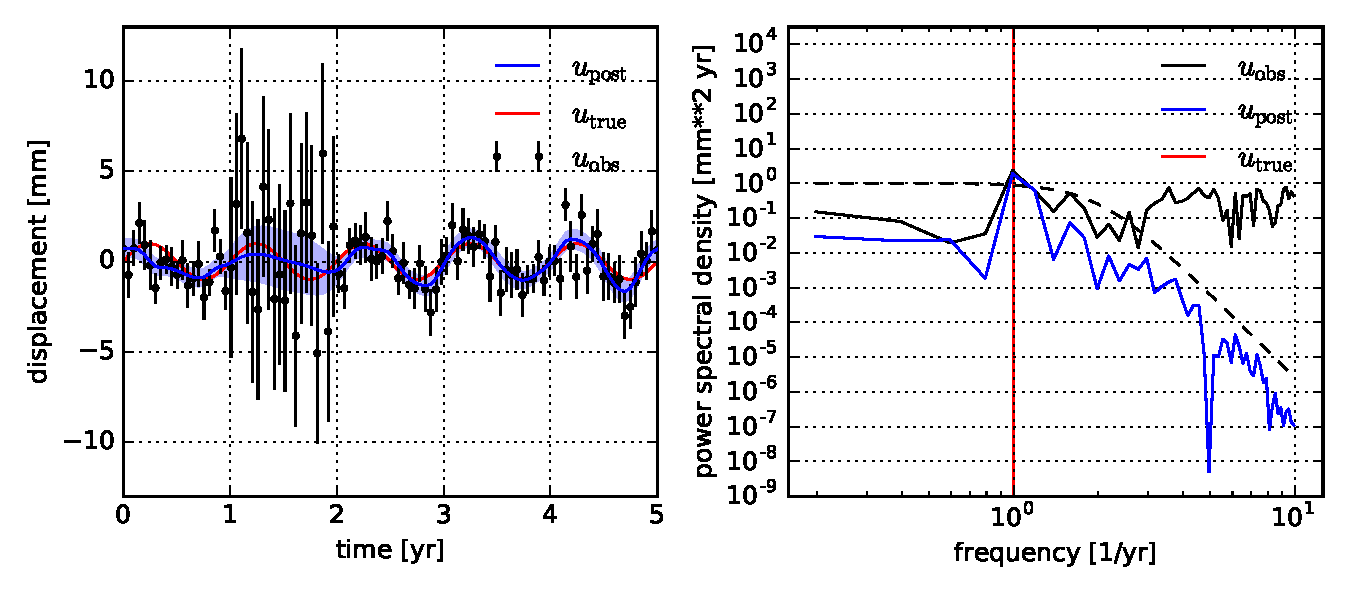
\includegraphics[scale=0.75]{figures/fig1}
\caption{Panel A shows $u_\mathrm{obs}$ (black scatter points), $u_\mathrm{post}$ (blue line), and the true signal which we are trying to recover (red line).  The lines on each scatter point and the light blue region show the one standard deviation uncertainty for the observations and filtered solution respectively. Panel B shows the estimated power spectral density for the observed, filtered, and true signal.  The black dashed line is the squared transfer function in eq. (\ref{eq:1DFourierSoln2}) with $\omega_c=2$ yr$^{-1}$, which roughly indicates how eq. (\ref{eq:1DSolution}) scales the frequency content of $u_\mathrm{obs}$.  If the data variances were constant then the frequency content of $u_\mathrm{obs}$ and $\bar{u}_\mathrm{post}$ would be exactly related by the black dashed line.}   
\label{fig:Demo1}
\end{figure}

We present a similar demonstration to show that eq. (\ref{eq:1DSolution}) effectively acts as a low-pass filter even when the observations are not uniformly spaced.  We take samples over the time interval $(0,10)$ yr, where the sampling rate is $0.05$ yr$^{-1}$ for the first 5 years and $0.0125$ yr$^{-1}$ for the last 5 years.  We use the same underlying signal from the previous demonstration and we add noise with a constant variance of $1$ mm$^2$.  We keep $n=2$ but since we are dealing with non-uniformly spaced data, we can no longer use the periodic spectral differentiation matrix, and $\mathbf{D}_n$ is instead a first-order accurate finite difference matrix for arbitrarily spaced data \citep{Fornberg1996}.  Once again, our cutoff frequency is $\omega_c = 2$ yr$^{-1}$.  The synthetic data and filtered solution are shown in panel A of Figure \ref{fig:Demo2}.  The power spectral density for the time intervals $(0,5)$ and $(5,10)$ yr are shown in panel B and C, respectively.  In both panels B and C, the spectral density of the filtered solution diverges from the spectral density of the synthetic observations at the expected cutoff frequency of $\omega_c$.  For frequencies above ${\sim}5$ yr$^{-1}$, the rate that the spectral content decays is slower than what is predicted by the transfer function in eq. (\ref{eq:1DFourierSoln2}). This is most pronounced in panel C, and we attribute the discrepancy to our lower order differentiation matrix. Barring the high frequencies which have negligable power in $\bar{u}_\mathrm{post}$, the power spectral density of $\bar{u}_\mathrm{post}$ relative to $u_\mathrm{obs}$ is accurately described by the transfer function in eq. (\ref{eq:1DFourierSoln2}), despite our use of non-uniform spacing.


\begin{figure}
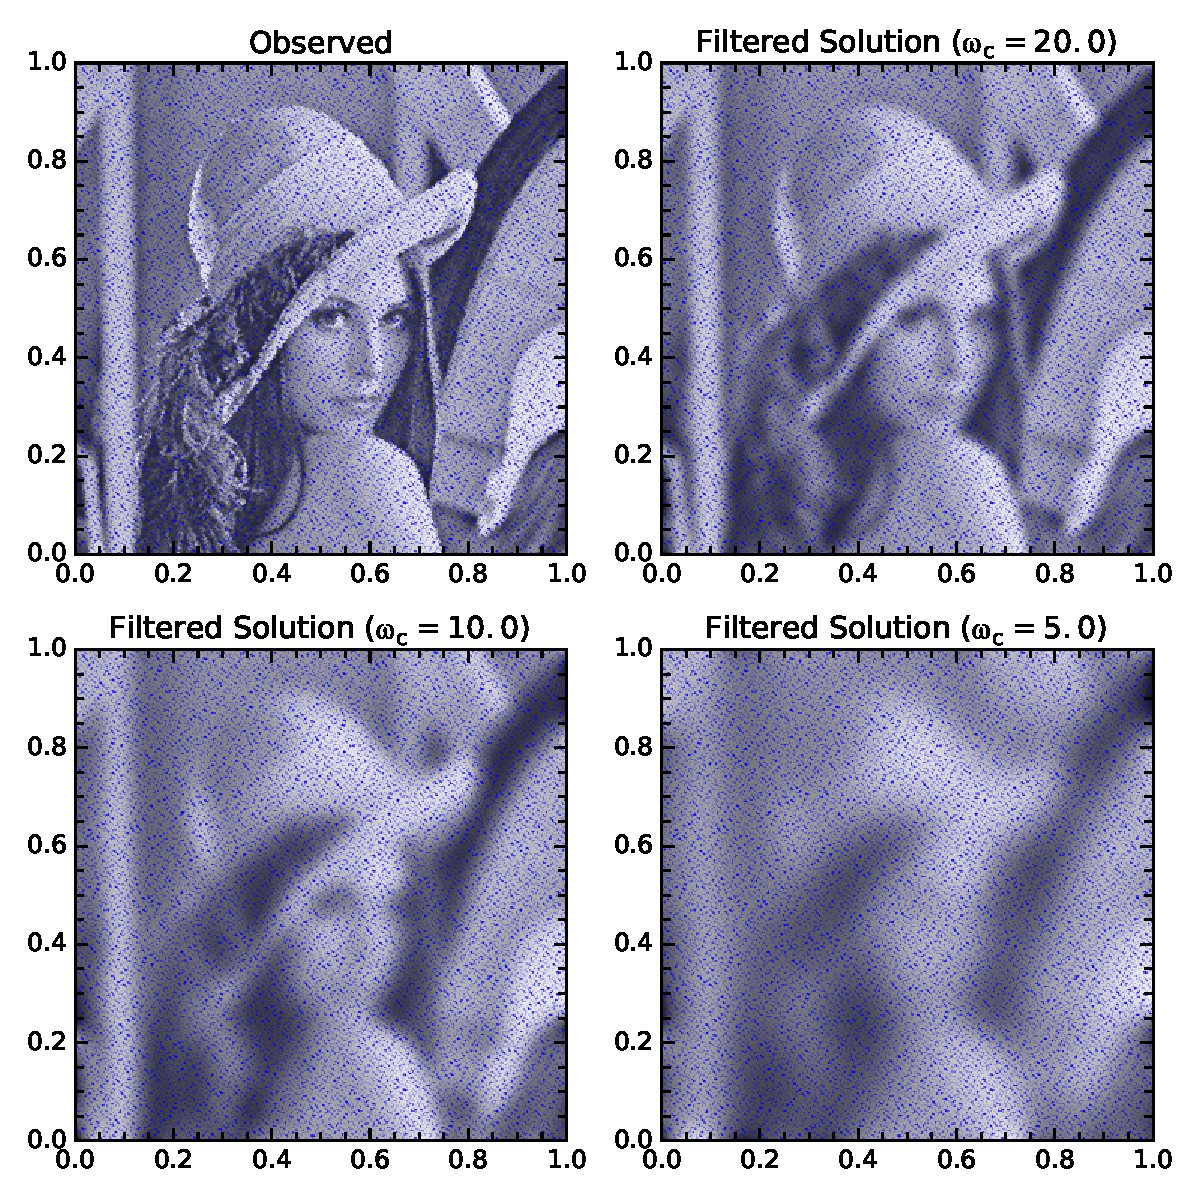
\includegraphics[scale=0.7]{figures/fig2}
\caption{Panel A shows $u_\mathrm{obs}$ (black scatter points), $u_\mathrm{post}$ (blue line), and the true signal which we are trying to recover (red line).  The light blue region show the one standard deviation uncertainty for $u_\mathrm{post}$. The uncertainties for the observations are all 1 mm and are not shown for the sake of clarity.  Panel B shows the estimated power spectral density for the observed, filtered, and true signal over the time interval (0,5) yr. Panel C is the same as panel B except for the time interval (5,10) yr.  In both panel B and C the black dashed line is the squared transfer function in eq. (\ref{eq:1DFourierSoln2}) with $\omega_c=2$ yr$^{-1}$.}   
\label{fig:Demo2}
\end{figure}

\section*{Smoothing in higher dimensions} 
We expand our discussion to smoothing data which is observed in $d$-dimensional space.  The filtered solution is still given by eq. (\ref{eq:GeneralSolution}), and we consider the prior model

\begin{equation}
  \mathbf{L}_n u_\mathrm{prior} = q, \ \ \ q \sim \mathcal{N}(0,\lambda^2)
\end{equation}  
where $\mathbf{L}_n$ is a differentiation matrix which approximates the operation 

\begin{equation}
  \sum_{i=1}^d\frac{\partial^n}{\partial x_i^n} 
\end{equation} 
and $n$ is an even integer. The corresponding covariance matrix is then

\begin{equation}\label{eq:NDCovariance}
\mathbf{C}_\mathrm{prior} = \lambda^2\left(\mathbf{L}_n^T\mathbf{L}_n\right)^{-1}. 
\end{equation}           
Using the change of variables from eq. (\ref{eq:VariableChange2}), the solution in the time domain is

\begin{equation}\label{eq:NDSolution}
\begin{split}
\bar{u}_\mathrm{post} &= (\mathbf{C}_\mathrm{obs}^{-1} +   
                   \frac{1}{(2\pi\omega_c)^{2n}\bar{\sigma}^2}\mathbf{L}_n^T\mathbf{L}_n)^{-1}\mathbf{C}_\mathrm{obs}^{-1}
                   u_\mathrm{obs}
\\
\mathbf{C}_\mathrm{post} &= (\mathbf{C}_\mathrm{obs}^{-1} +   
                            \frac{1}{(2\pi\omega_c)^{2n}\bar{\sigma}^2}\mathbf{L}_n^T\mathbf{L}_n)^{-1}.
\end{split}
\end{equation}
If we again assume that the observation have constant variance and $L_n$ is the corresponding spectral differentiation matrix, then the d-dimensional discrete Fourier transform of $\bar{u}_\mathrm{post}$ is 

\begin{equation}\label{eq:NDFourierSoln}
  \hat{u}_\mathrm{post}(\omega_1, \dots, \omega_d) = 
  \frac{1}{1 + \left(\sum_{i=1}^d \left(\frac{\omega_i}{\omega_c}\right)^n\right)^2} \hat{u}_\mathrm{obs}.
\end{equation}
The transfer function in eq. (\ref{eq:NDFourierSoln}) can once again be recognized as a low-pass filter.  Namely, in the limit as $n \to \infty$, the transfer function becomes a $d$-dimensional box which is zero for all the frequency tuples, $(\omega_1,\dots,\omega_n)$, which have a component greater than $\omega_c$. 

\bibliographystyle{apalike}
\bibliography{mybib}  
 
\end{document}